\documentclass[11pt]{article}

% ============================================================
% PACKAGES AND PAGE STYLE
% ============================================================

\usepackage[a4paper,margin=1in]{geometry}
\usepackage{amsmath,amssymb}
\usepackage{booktabs}
\usepackage{graphicx}
\usepackage{xcolor}
\usepackage{fancyhdr}
\usepackage{hyperref}
\usepackage{listings}

\definecolor{UFBlue}{HTML}{0021A5}
\definecolor{UFOrange}{HTML}{FA4616}
\definecolor{DarkGray}{HTML}{333333}
\definecolor{LightGray}{HTML}{F4F4F4}

\hypersetup{
    colorlinks=true,
    linkcolor=UFBlue,
    urlcolor=UFBlue,
    citecolor=UFBlue,
    pdftitle={COT5405 Project: Greedy Scheduling and Divide-and-Conquer FFT},
    pdfauthor={Pradhyuman Singh Shekhawat}
}

\setlength{\parindent}{0pt}
\setlength{\parskip}{5pt}
\setlength{\headheight}{15pt}

\pagestyle{fancy}
\fancyhf{}
\fancyhead[L]{\small\textcolor{UFBlue}{COT5405 --- Analysis of Algorithms}}
\fancyhead[R]{\small\textcolor{DarkGray}{Course Project}}
\fancyfoot[C]{\small\thepage}
\renewcommand{\headrulewidth}{0.5pt}

\newcommand{\code}[1]{\texttt{\detokenize{#1}}}

\lstset{
    basicstyle=\ttfamily\small,
    backgroundcolor=\color{LightGray},
    frame=single,
    breaklines=true,
    columns=fullflexible,
    keepspaces=true,
    showstringspaces=false
}

\begin{document}

% ============================================================
% TITLE PAGE
% ============================================================

\begin{titlepage}
\thispagestyle{empty}
\begin{center}

\vspace*{0.35in}

\IfFileExists{ufl-logo.png}{
    
\includegraphics[width=5in]{ufl-logo.png}
}{
    {\Large\textcolor{UFBlue}{\textbf{UNIVERSITY OF FLORIDA}}}\\[2mm]
    {\color{UFOrange}\rule{2.65in}{1.2pt}}
}

\vspace{0.65in}

{\Large\textcolor{UFBlue}{\textbf{COT5405 --- ANALYSIS OF ALGORITHMS}}}

\vspace{0.18in}

{\Huge\bfseries\textcolor{DarkGray}{Project - 1}}

\vspace{0.10in}

{\LARGE\bfseries\textcolor{UFBlue}{Greedy Scheduling and Divide-and-Conquer FFT}}

\vspace{0.30in}

{\color{UFOrange}\rule{4.6in}{1.5pt}}

\vspace{0.45in}

{\large
\begin{tabular}{r l}
\textbf{Student:} & Pradhyuman Singh Shekhawat\\
\textbf{UFID:} & 55742970\\
\textbf{Email:} & pr.shekhawat@ufl.edu\\
\textbf{Term:} & Fall 2026\\
\textbf{Components:} & Greedy scheduling and radix-2 FFT\\
\end{tabular}
}

\vfill

{\small University of Florida\\[2pt]\today}

\end{center}
\end{titlepage}

\pagenumbering{roman}
\tableofcontents
\clearpage
\pagenumbering{arabic}

% ============================================================
\section{Introduction}

This project studies two algorithmic techniques through separate
application problems. The first is a greedy algorithm that selects a
maximum-cardinality set of mutually compatible communication intervals
from a fixed candidate set. The second is a divide-and-conquer radix-2
Cooley--Tukey Fast Fourier Transform (FFT) for computing the discrete
Fourier transform of sampled vibration signals.

For each component, the report defines the application and mathematical
problem, describes the algorithm, analyzes its running time, proves
correctness, and presents implementation and empirical validation.
The scheduling result is optimal only for the supplied fixed interval
set; it does not solve the full multi-resource Deep Space Network
scheduling problem. The FFT computes a spectrum and is not itself a
bearing-fault classifier.

% ============================================================
\section{Greedy Algorithm: Communication-Interval Scheduling}

\subsection{Application and Problem Definition}

Deep-space communication planning must respect antenna availability
and non-overlapping use of a resource. This project uses candidate
communication intervals associated with antenna DSS-34. For the
algorithmic abstraction, each candidate interval has a start time and
finish time, and all intervals have equal value. The objective is to
select the largest number of pairwise non-overlapping intervals.

Intervals are interpreted as half-open intervals $[s_i,f_i)$;
therefore, one interval ending exactly when another begins is
compatible. This is a simplified single-resource abstraction, not a
complete model of operational Deep Space Network scheduling.

\subsection{Mathematical Abstraction}

Let $I=\{1,\ldots,n\}$ be the set of candidate intervals. Interval $i$
has start time $s_i$ and finish time $f_i$, where $s_i<f_i$. A feasible
set $S\subseteq I$ satisfies, for every distinct pair $i,j\in S$,
either $f_i\leq s_j$ or $f_j\leq s_i$. The objective is

\[
\max |S|
\quad \text{subject to } S \text{ being feasible}.
\]

The unit-value assumption is important: maximizing the number of
intervals does not necessarily maximize total communication duration
or scientific value.

\subsection{Algorithm}

Sort intervals in nondecreasing order of finish time. Select the first
interval, then scan the remaining sorted intervals and select interval
$i$ whenever $s_i\geq f_{\mathrm{last}}$, where
$f_{\mathrm{last}}$ is the finish time of the most recently selected
interval.

\newpage

\begin{lstlisting}[language=Python,caption={Earliest-finish-time greedy algorithm (pseudocode)}]
sort intervals by nondecreasing finish time

selected = []
last_finish = -infinity

for interval in intervals:
    if interval.start >= last_finish:
        selected.append(interval)
        last_finish = interval.finish

return selected
\end{lstlisting}

\subsection{Correctness Proof}

Let $g$ be an interval with the earliest finish time among all
available intervals. Let $O$ be an optimal solution, and let $o$ be
its first interval. Since $f_g\leq f_o$, replacing $o$ with $g$
preserves feasibility for every later interval in $O$: any interval
that starts at or after $f_o$ also starts at or after $f_g$.
Thus, there exists an optimal solution that begins with $g$.

After selecting $g$, the remaining compatible intervals all start at
or after $f_g$. The same argument applies to this remaining subproblem.
Repeating the exchange argument proves that each greedy choice can be
part of an optimal solution, so the algorithm returns a
maximum-cardinality feasible subset.

This proof applies to the fixed candidate intervals and the
unit-value objective defined above, not to arbitrary weighted
scheduling or the full DSN problem.

\subsection{Running-Time Analysis}

Sorting takes $O(n\log n)$ time. The subsequent scan takes $O(n)$
time, so the total running time is $O(n\log n)$, dominated by sorting.
Storing the sorted intervals and selected set requires $O(n)$ space
in the implementation.

\subsection{Audit and Scheduling Results}

The audit pipeline reported 1,452 requests and 874 candidate intervals
for DSS-34, corresponding to 60.193\% of the requests. The scheduler
selected 119 intervals and skipped 755 conflicting candidates.
The selected interval counts by week were W10: 27, W20: 21, W30: 24,
W40: 24, and W50: 23.

These figures describe the current pipeline output and should not be
interpreted as a global optimum over every possible visibility
opportunity. The greedy algorithm is optimal on the fixed candidate
interval set supplied to it, under the maximum-cardinality objective.

\subsection{Correctness and Feasibility Validation}

The implementation was tested using unit tests and an independent
optimality checker. The checker compared the greedy algorithm's
selection count with a dynamic-programming solution on 1,000 randomly
generated small interval sets. The corrected checker reported matching
optimal values for those test instances.

A feasibility check of the selected schedule reported zero overlap
violations among the 119 selected intervals. These tests provide
evidence for the implementation's correctness on the tested inputs;
they do not replace the mathematical correctness proof or establish
optimality for the full operational DSN scheduling problem.

\subsection{Greedy Runtime Measurements}

The repository contains runtime benchmark artifacts under
\code{greedy_dsn/results/runtime/}. The CSV file and plot generated
by the final benchmark run should be retained with the project.

\begin{figure}[ht]
\centering
\IfFileExists{../../greedy_dsn/results/runtime/runtime_median.png}{
    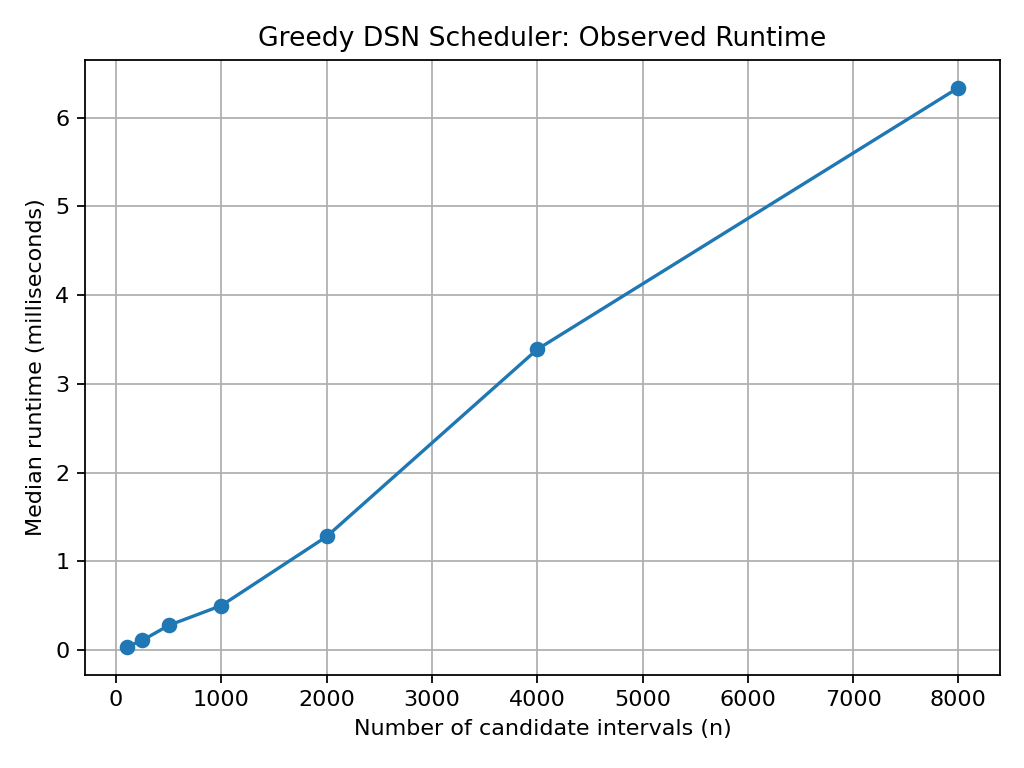
\includegraphics[width=0.82\textwidth]
    {../../greedy_dsn/results/runtime/runtime_median.png}
}{
    \fbox{\parbox{0.82\textwidth}{\centering
    Greedy runtime plot not found. Check the relative path to
    \code{runtime_median.png}.}}
}
\caption{Measured runtime of the greedy scheduling implementation.}
\label{fig:greedy-runtime}
\end{figure}

The expected asymptotic running time is $O(n\log n)$, primarily
because the intervals must be sorted. The benchmark plot provides
empirical evidence about the implementation on the tested machine.
Observed timings can vary because of interpreter overhead, system
load, and input characteristics.

% ============================================================
\section{Divide-and-Conquer Algorithm: Bearing-Vibration FFT}

\subsection{Application and Scope}

Vibration sensors record sampled time-domain signals from rotating
machinery. Transforming these samples into the frequency domain helps
engineers inspect prominent frequency components. The Case Western
Reserve University Bearing Data Center provides documented bearing
vibration measurements and experimental conditions \cite{cwru}.

An FFT is a signal-processing step only: a spectrum does not by itself
diagnose a bearing fault or classify its type.

\subsection{Mathematical Abstraction}

Given a sequence $x[0],\ldots,x[n-1]$ with $n=2^k$, compute its
discrete Fourier transform (DFT):

\[
X[m]=\sum_{j=0}^{n-1}x[j]e^{-2\pi i jm/n},
\qquad m=0,\ldots,n-1.
\]

Here $x[j]$ is a time-domain sample and $X[m]$ is the complex
coefficient at frequency bin $m$. For sample rate $f_s$, the bin
spacing is $f_s/n$ Hz.

\subsection{Divide-and-Conquer Algorithm}

Separate the input into even- and odd-indexed subsequences:
$x_e[r]=x[2r]$ and $x_o[r]=x[2r+1]$. Recursively compute their
length-$n/2$ DFTs, denoted by $E[m]$ and $O[m]$. With
$W_n^m=e^{-2\pi i m/n}$, combine:

\[
X[m]=E[m]+W_n^mO[m],
\]

\[
X[m+n/2]=E[m]-W_n^mO[m],
\]

for $0\leq m<n/2$. The base case is a one-element sequence. The
implementation rejects empty input and lengths that are not powers
of two.

\subsection{Correctness Proof}

Split the DFT sum into even and odd indices:

\[
\begin{aligned}
X[m]
={}&\sum_{r=0}^{n/2-1}x[2r]e^{-2\pi i(2r)m/n}\\
&+\sum_{r=0}^{n/2-1}x[2r+1]e^{-2\pi i(2r+1)m/n}.
\end{aligned}
\]

The first sum is $E[m]$. Factoring $e^{-2\pi i m/n}$ from the second
sum makes it $W_n^mO[m]$, hence

\[
X[m]=E[m]+W_n^mO[m].
\]

For the coefficient at $m+n/2$, the even-index exponential is
unchanged, while the odd-index exponential acquires a factor of
$e^{-\pi i}=-1$. Therefore,

\[
X[m+n/2]=E[m]-W_n^mO[m].
\]

For $n=1$, the algorithm returns the input, which is its DFT. Assume
the recursive calls correctly compute the DFTs of length $n/2$.
The derived combination equations then produce all $n$ DFT
coefficients correctly. Induction on powers of two proves correctness
for every accepted input length.

\subsection{Running-Time Analysis}

At each recursion level, two subproblems of size $n/2$ are solved
and the combination step performs $\Theta(n)$ work. Thus,

\[
T(n)=2T(n/2)+\Theta(n),
\qquad T(1)=\Theta(1).
\]

By the Master Theorem, $T(n)=\Theta(n\log n)$. This recursive
implementation uses $O(n)$ auxiliary space across its lists and
recursive computations.

\subsection{Correctness Tests and Synthetic Demonstration}

Seven unit tests passed. They check the one-sample base case,
constant and impulse signals, a sinusoid with a known frequency bin,
comparison with a direct DFT on deterministic random inputs, and
rejection of invalid input lengths.

The synthetic demonstration used $n=1024$ samples at $f_s=1024$ Hz,
giving 1 Hz bin spacing. The largest magnitudes appeared at 64 Hz,
180 Hz, and 230 Hz, as expected from the generated signal. These
results validate the implementation on controlled inputs; they are
not results from a real bearing recording.

\subsection{Empirical Runtime Results}

Table~\ref{tab:fft-runtime} reports the measured median runtime from
seven repetitions on the tested machine. These are synthetic-input
timings.

\begin{table}[ht]
\centering
\caption{Radix-2 FFT median runtime (seven repetitions).}
\label{tab:fft-runtime}
\begin{tabular}{rr}
\toprule
Input size $n$ & Median runtime (ms)\\
\midrule
256    & 0.5455\\
512    & 1.1579\\
1,024  & 2.5629\\
2,048  & 5.7415\\
4,096  & 13.2173\\
8,192  & 24.4893\\
16,384 & 51.8880\\
32,768 & 109.8920\\
\bottomrule
\end{tabular}
\end{table}

\begin{figure}[ht]
\centering
\IfFileExists{../../divide_conquer_fft/results/fft_runtime_vs_nlogn.png}{
    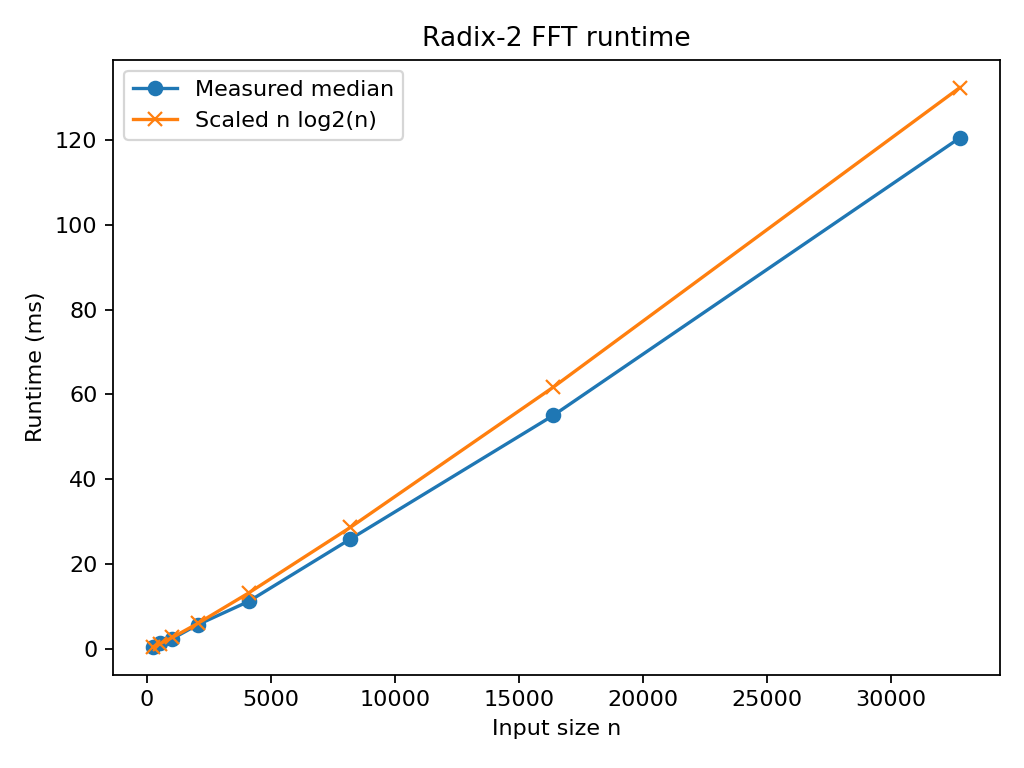
\includegraphics[width=0.82\textwidth]
    {../../divide_conquer_fft/results/fft_runtime_vs_nlogn.png}
}{
    \fbox{\parbox{0.82\textwidth}{\centering
    FFT runtime plot not found. Check the relative path to
    \code{fft_runtime_vs_nlogn.png}.}}
}
\caption{Measured FFT runtime compared with a scaled $n\log_2 n$ curve.}
\label{fig:fft-runtime}
\end{figure}

The measured runtime increases with input size and broadly follows
the expected $n\log n$ growth. Deviations from the scaled reference
curve can arise from Python recursion and list-allocation overhead,
interpreter behavior, and machine load. The recurrence, rather than
the timing plot, establishes the asymptotic bound.

\subsection{Real-Data Demonstration}

The FFT implementation was also evaluated on a vibration recording
from the Case Western Reserve University Bearing Data Center
\cite{cwru}. The input file was \code{data/105.mat}, and the selected
channel was \code{X105_DE_time}. The first 4,096 samples were used
with a sampling rate of 12,000 Hz. The mean was removed from the
segment before computing the spectrum.

The resulting frequency resolution was

\[
\Delta f=\frac{f_s}{n}
=\frac{12000}{4096}
\approx 2.93\text{ Hz}.
\]

The largest reported spectral magnitudes occurred near 3585.94 Hz,
2616.21 Hz, and 2879.88 Hz. These values describe peaks in the
processed segment; they are not, by themselves, evidence of a
specific bearing defect.

\begin{figure}[ht]
\centering
\IfFileExists{../../divide_conquer_fft/results/real_data/105_waveform.png}{
    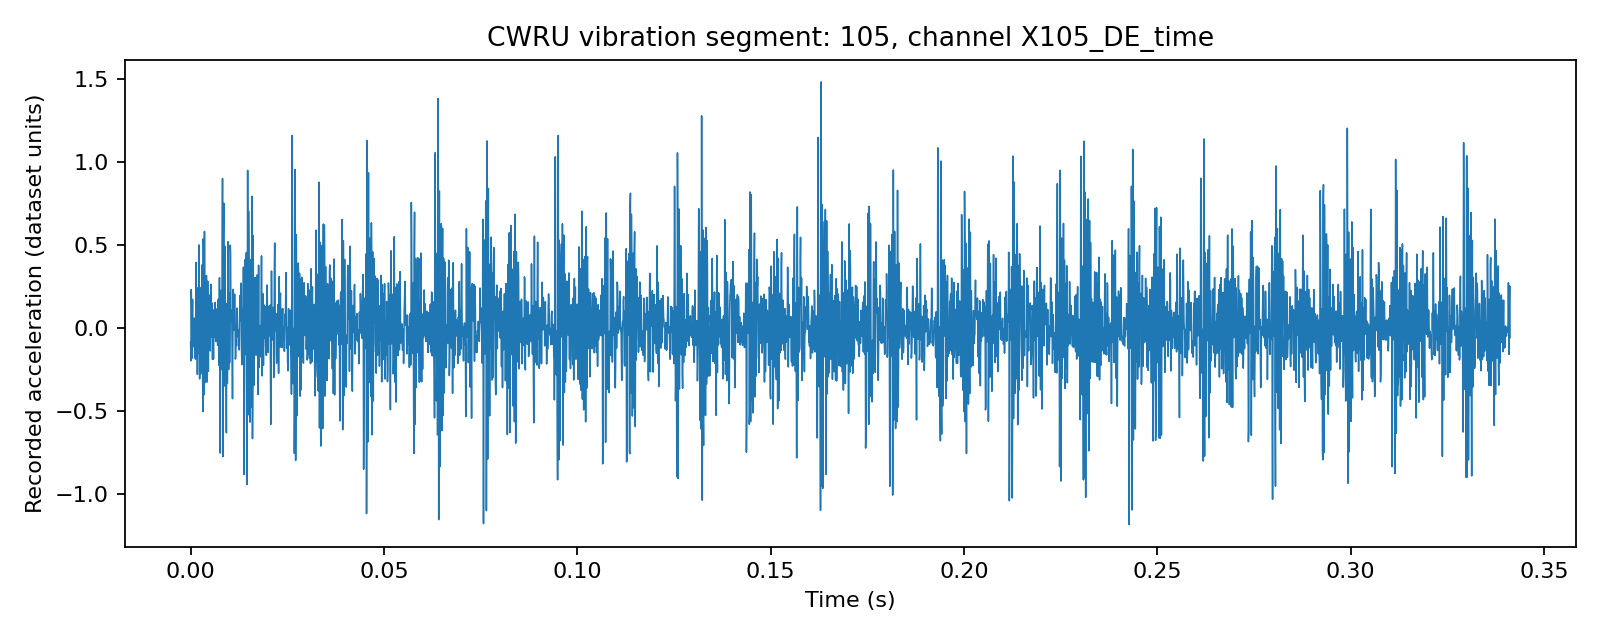
\includegraphics[width=0.82\textwidth]
    {../../divide_conquer_fft/results/real_data/105_waveform.png}
}{
    \fbox{\parbox{0.82\textwidth}{\centering
    Real-data waveform plot not found. Check the path to
    \code{105_waveform.png}.}}
}
\caption{Time-domain waveform for the selected segment of channel
\code{X105_DE_time}.}
\label{fig:real-waveform}
\end{figure}

\begin{figure}[ht]
\centering
\IfFileExists{../../divide_conquer_fft/results/real_data/105_spectrum.png}{
    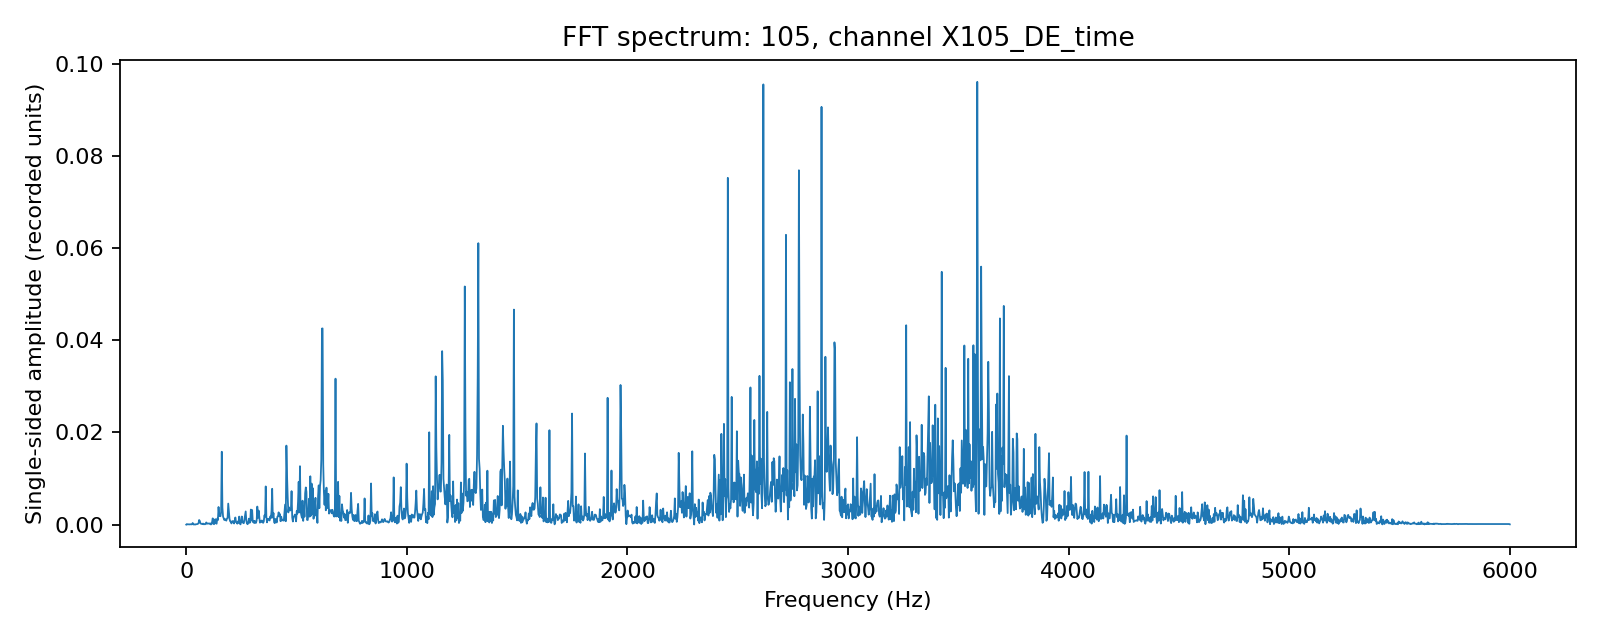
\includegraphics[width=0.82\textwidth]
    {../../divide_conquer_fft/results/real_data/105_spectrum.png}
}{
    \fbox{\parbox{0.82\textwidth}{\centering
    Real-data spectrum plot not found. Check the path to
    \code{105_spectrum.png}.}}
}
\caption{FFT magnitude spectrum of the selected real vibration segment.}
\label{fig:real-spectrum}
\end{figure}

The synthetic benchmark and real-data demonstration serve different
purposes. The synthetic signal provides known frequency components
for checking expected behavior, while the real recording demonstrates
processing of an experimental vibration signal. The spectrum is an
analytical output, not a diagnosis or a classification result.

% ============================================================
\section{Comparison and Discussion}

The greedy algorithm makes locally optimal choices supported by an
exchange argument and solves a maximum-cardinality interval-selection
problem in $O(n\log n)$ time. The FFT recursively decomposes the DFT
and combines partial solutions using roots of unity, achieving
$O(n\log n)$ time.

Although both bounds share the same asymptotic form, they describe
different operations and input models. Their empirical results should
not be compared directly because the measured workloads and units of
work differ.

The greedy algorithm's correctness guarantee depends on the
fixed-candidate, single-resource, equal-value interval abstraction.
The FFT's correctness guarantee applies to accepted power-of-two
input lengths and follows from the DFT decomposition and induction.
In both cases, theoretical analysis and empirical testing play
complementary roles.

% ============================================================
\section{Limitations and Future Work}

The scheduling model assumes a fixed candidate interval set, a
single antenna, and equal value per interval. It omits global
optimization over all visibility opportunities and broader operational
constraints. Future work could examine more realistic resource
constraints, multiple antennas, and objectives that account for
communication duration or scientific value. Such extensions would
require a separate algorithmic formulation and correctness analysis.

The FFT implementation uses radix-2 recursion and therefore accepts
only input lengths that are powers of two. The benchmark measures
execution time on one machine, and the observed timings may vary
across environments. Future work could compare the implementation
against a trusted numerical library and examine larger or differently
structured signals.

The real-data demonstration uses one selected channel and one segment.
Its spectral peaks should not be treated as a bearing diagnosis.
Interpreting the condition of machinery would require additional
domain-specific analysis and supporting evidence.

% ============================================================
\section{Use of AI Tools}

AI assistance was used during project development for algorithm
discussion, implementation review, test development, debugging, and
report drafting. The final appendix should document the actual prompts
and relevant outputs required by the course policy. The following
table summarizes the main types of assistance and the verification
work that should be documented.

\begin{table}[ht]
\centering
\caption{AI-use and verification summary.}
\small
\begin{tabular}{p{0.18\textwidth}p{0.34\textwidth}p{0.36\textwidth}}
\toprule
Task & AI assistance used & Verification and refinement\\
\midrule
Greedy algorithm &
Discussion of interval scheduling, algorithm design, and correctness
reasoning. &
Unit tests, independent dynamic-programming comparison on 1,000
random small instances, and a schedule overlap check.\\
\midrule
FFT algorithm &
Discussion of radix-2 FFT design, recurrence, correctness, and test
cases. &
Seven unit tests, direct-DFT comparisons, and a synthetic-frequency
check.\\
\midrule
Report drafting &
Organization and refinement of technical explanations and LaTeX
formatting. &
Review proofs, citations, code paths, runtime values, plots, and
real-data claims against the project artifacts.\\
\bottomrule
\end{tabular}
\end{table}

This summary is not a substitute for the exact prompt/output log if
the assignment requires it. Exact prompts should be copied from the
actual conversation history rather than reconstructed and presented
as verbatim records.

% ============================================================
\appendix

\section{Runtime-Validation Code}

The greedy runtime benchmark is maintained in
\code{greedy_dsn/scripts/benchmark_greedy_runtime.py}, and the FFT
runtime benchmark is maintained in
\code{divide_conquer_fft/scripts/benchmark_fft.py}.

The corresponding CSV files and generated plots should be retained
with the submission. The runtime results in this report should match
the exact benchmark outputs included in the final project.

\newpage

\section{Reproducibility Commands}

Run the following commands from the repository root unless otherwise
specified.

\begin{lstlisting}
# Run greedy tests
python -m unittest discover \
    -s greedy_dsn/tests -p 'test_*.py' -v

# Check greedy optimality on random small instances
python greedy_dsn/tests/verify_greedy_optimality.py

# Run the greedy audit
python greedy_dsn/scripts/audit_satnet_v2.py \
    --problems greedy_dsn/data/problems.json \
    --maintenance greedy_dsn/data/maintenance.csv \
    --antenna DSS-34 \
    --out greedy_dsn/results/audit_v2

# Run the greedy scheduler
python greedy_dsn/src/greedy_satnet.py \
    --input greedy_dsn/results/audit_v2/candidate_intervals.csv \
    --out greedy_dsn/results/schedule
\end{lstlisting}

Run the FFT commands from the \code{divide_conquer_fft} directory:

\begin{lstlisting}
# Run FFT tests
python -m unittest discover -s tests -v

# Run the FFT benchmark
python scripts/benchmark_fft.py \
    --out results \
    --min-power 8 \
    --max-power 15 \
    --repeats 7

# Run the real-data demonstration
python scripts/demo_real_data.py \
    --file data/105.mat \
    --sample-rate 12000 \
    --channel auto \
    --samples 4096 \
    --out results/real_data
\end{lstlisting}

% ============================================================
\newpage

\begin{thebibliography}{9}

\bibitem{cwru}
Case Western Reserve University.
\newblock \emph{Bearing Data Center}.
\newblock Available at:
\url{https://engineering.case.edu/bearingdatacenter}.

\bibitem{cooley-tukey}
James W. Cooley and John W. Tukey.
\newblock An algorithm for the machine calculation of complex Fourier series.
\newblock \emph{Mathematics of Computation}, 19(90):297--301, 1965.
\newblock \url{https://doi.org/10.1090/S0025-5718-1965-0178586-1}.

\bibitem{nasa-dsn}
NASA Technical Reports Server.
\newblock Deep Space Network scheduling research resources.
\newblock Available at:
\url{https://ntrs.nasa.gov/citations/20230006929}.

\end{thebibliography}

\end{document}